\documentclass{clbeamer2024}

\usepackage{minted}

\usepackage{minted}
\setminted{
	breaklines=true,
	frame=single,
	bgcolor=lightgray,
	fontsize=\small,
	escapeinside=||
}

\usepackage{xcolor}
\definecolor{bg}{rgb}{0.95, 0.95, 0.92} % Couleur gris clair

\title{
	%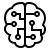
\includegraphics[width=0.5cm]{logos/IA1.png} \hfill
        Introduction à MongoDB
	
\includegraphics[width=0.7cm]{logos/MongoDB.png} \hfill
}
\subtitle{Comprendre les bases de la base de données NoSQL orientée documents}
\author{Slimani Mohamed Amine}
\institute{EHTP}
\date{\today}

\begin{document}
	\setcounter{framenumber}{-1}
	\frame{\titlepage}
	
	
	
	% Sommaire
	\begin{frame}{Sommaire}
		\tableofcontents
	\end{frame}
	
	
	\section{Qu'est-ce que MongoDB ?}
	\begin{frame}{Qu'est-ce que MongoDB ?}
		\begin{itemize}
			\item \textbf{Définition} : MongoDB est une base de données NoSQL orientée documents, qui stocke les données sous forme de documents JSON-like (BSON).
			\item \textbf{Objectif} : Offrir une solution de stockage flexible et scalable pour les applications modernes.
			\item \textbf{Avantages} : Flexibilité, scalabilité, performances élevées.
		\end{itemize}
	\end{frame}
	
	
	\section{Pourquoi utiliser MongoDB ?}
	\begin{frame}{Pourquoi utiliser MongoDB ?}
		\begin{itemize}
			\item \textbf{Flexibilité} : Pas de schéma fixe, adapté aux données non structurées ou semi-structurées.
			\item \textbf{Scalabilité} : Facile à scaler horizontalement avec le sharding.
			\item \textbf{Performances} : Accès rapide aux données grâce à l'indexation.
		\end{itemize}
	\end{frame}
	
	
	\section{Concepts de base de MongoDB}
	\begin{frame}{Concepts de base de MongoDB}
		\begin{itemize}
			\item \textbf{Document} : Unité de base de données, stockée en BSON (Binary JSON).
			\item \textbf{Collection} : Groupe de documents, similaire à une table dans les bases de données relationnelles.
			\item \textbf{Base de données} : Conteneur pour les collections.
		\end{itemize}
	\end{frame}	
	
	
	\section{Architecture de MongoDB}
	\begin{frame}{Architecture de MongoDB}
		\begin{itemize}
			\item \textbf{Moteur de stockage} : WiredTiger (par défaut) pour la gestion des données.
			\item \textbf{Sharding} : Répartition des données sur plusieurs serveurs pour la scalabilité.
			\item \textbf{Réplication} : Copie des données sur plusieurs serveurs pour la haute disponibilité.
		\end{itemize}
	\end{frame}
	
	
\section{Bonnes pratiques}
\begin{frame}{Bonnes pratiques}
	\begin{itemize}
		\item \textbf{Indexation} : Créer des index pour accélérer les requêtes.
		\item \textbf{Schéma flexible} : Profiter de la flexibilité tout en gardant une structure logique.
		\item \textbf{Sécurité} : Configurer l'authentification et le chiffrement.
	\end{itemize}
\end{frame}
	
	
	\section{Outils pour travailler avec MongoDB}
	\begin{frame}{Outils pour travailler avec MongoDB}
		\begin{itemize}
			\item \textbf{MongoDB Compass} : Interface graphique pour interagir avec MongoDB.
			\item \textbf{MongoDB Atlas} : Service cloud pour déployer et gérer MongoDB.
			\item \textbf{Mongoose} : Bibliothèque ODM (Object Data Modeling) pour Node.js.
		\end{itemize}
	\end{frame}
	

	
	\section{Exemple d'application avec MongoDB et Node.js}
	\begin{frame}{Exemple d'application avec MongoDB et Node.js}
		\begin{exampleblock}{Connexion à MongoDB avec Node.js}
			\begin{center}
			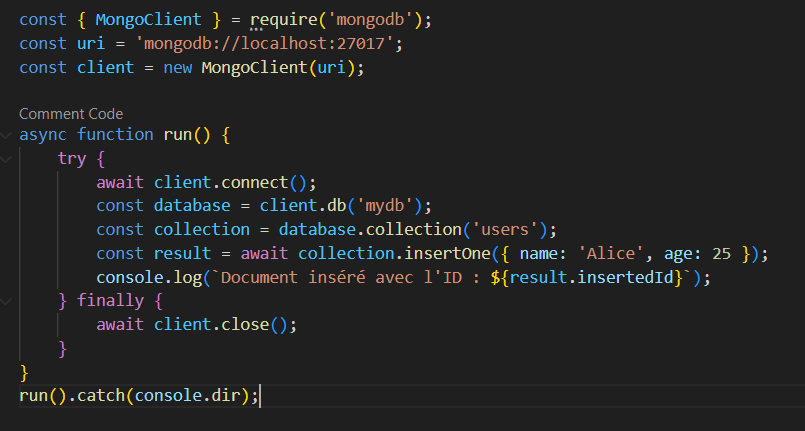
\includegraphics[width=0.87\textwidth]{images/code1.png}
		\end{center}
		\end{exampleblock}
	\end{frame}
	
	
	\section{Défis de MongoDB}
	\begin{frame}{Défis de MongoDB}
		\begin{itemize}
			\item \textbf{Gestion des schémas} : Bien que flexible, un schéma mal conçu peut entraîner des problèmes de performance.
			\item \textbf{Consommation de mémoire} : MongoDB peut utiliser beaucoup de mémoire pour les grandes bases de données.
			\item \textbf{Sécurité} : Configuration correcte nécessaire pour éviter les vulnérabilités.
		\end{itemize}
	\end{frame}
	
	
	\section{Pourquoi c'est important ?}
	\begin{frame}{Pourquoi c'est important ?}
		\begin{itemize}
			\item MongoDB est une base de données puissante pour les applications modernes.
			\item Elle offre flexibilité, scalabilité, et performances élevées.
			\item Comprendre MongoDB est essentiel pour les développeurs et les administrateurs de bases de données.
		\end{itemize}
	\end{frame}
	
	
	\begin{frame}{Résumé}
		\textbf{MongoDB} est une base de données NoSQL révolutionnaire pour le stockage flexible et scalable des données.  
		Explorez, apprenez, et innovez avec MongoDB !
	\end{frame}
	
\end{document}
